\subsubsection{Algoritmo de detección de cintas}

El algoritmo de detección de cintas de referencia explota el alto contraste entre la cinta negra y el fondo claro mediante procesamiento en el canal de valor (V) del espacio HSV. Esta elección se fundamenta en la invariancia del canal V ante cambios en la tonalidad cromática de la iluminación, propiedad demostrada en el marco teórico (Sección 2.2.1).\\

Etapa 1: Conversión al espacio HSV:\\
\noindent
El proceso inicia con la captura de una imagen RGB de la región donde se espera encontrar el marcador. La imagen se transforma al espacio HSV aplicando las ecuaciones de conversión estándar, y se extrae el canal V que representa el brillo de cada píxel.\\

Etapa 2: Umbralización inversa\\
\noindent
Sobre el canal V se aplica umbralización inversa con valor de referencia de 50, operación que asigna valor máximo (blanco) a los píxeles oscuros y valor nulo (negro) a los píxeles claros. Matemáticamente:

\begin{equation}
I_{bin}(x,y) = \begin{cases}
255 & \text{si } I_V(x,y) < 50 \\
0 & \text{si } I_V(x,y) \geq 50
\end{cases}
\end{equation}

El valor de umbral 50 se determinó experimentalmente mediante análisis del imágenes representativas, identificando el punto que maximiza la separación entre la distribución de intensidades de las cintas negras y la distribución de intensidades del fondo blanco.\\

Etapa 3: Detección de contornos\\
\noindent
Sobre la imagen binaria resultante se ejecuta el algoritmo de detección de contornos de Suzuki-Abe, obteniendo las fronteras de todas las regiones oscuras detectadas. Los contornos se filtran aplicando un criterio de área mínima de 500 píxeles, eliminando elementos espurios correspondientes a ruido o pequeñas sombras. Este umbral se estableció considerando que una cinta de 18 milímetros de ancho a 200 milímetros de distancia subtiende aproximadamente 120 píxeles de ancho en la imagen, resultando en áreas típicas superiores a 3000 píxeles para segmentos de cinta de longitud razonable.

\subsubsection{Evaluación de calidad del contorno}

Los contornos que superan el filtrado de área se someten a evaluación de calidad para discriminar entre cintas de referencia genuinas y otros elementos oscuros presentes en la escena (como plantas o vasos). La evaluación se basa en el análisis de la región basal del contorno, definida como el 10 por ciento inferior de su rectángulo delimitador.

Para cada contorno candidato se calcula su rectángulo delimitador $(x, y, w, h)$, donde $(x,y)$ representa la esquina inferior izquierda, $w$ el ancho y $h$ la altura. La región basal se define entonces como:

\begin{equation}
R_{base} = \{(x',y') : x \leq x' < x+w, \, y+0.9h \leq y' < y+h\}
\end{equation}

Se calcula la fracción de píxeles blancos en esta región respecto al total de píxeles de la región:

\begin{equation}
Q_{base} = \frac{1}{|R_{base}|} \sum_{(x,y) \in R_{base}} \frac{I_{bin}(x,y)}{255}
\end{equation}

donde $|R_{base}|$ denota el número de píxeles en la región. Un valor $Q_{base}$ cercano a 1 indica que la región basal del contorno es consistentemente oscura, característica de las cintas de referencia cuyo borde inferior es nítido y bien definido. Valores inferiores indican contornos de objetos con bases irregulares o discontinuas, como plantas con hojas que no presentan un borde horizontal claro.

Esta métrica resulta efectiva para distinguir cintas de otros elementos oscuros: las cintas genuinas presentan típicamente $Q_{base} > 0.8$, mientras que plantas u otros objetos tienen $Q_{base} < 0.5$. Se establece un umbral de aceptación de 0.7 como compromiso entre sensibilidad y especificidad.

\subsubsection{Sistema de evaluación ponderada}

Cuando múltiples contornos cumplen los criterios de área mínima y calidad basal, se implementa un sistema de evaluación ponderada que considera tres factores para seleccionar el mejor candidato.

El primer factor evalúa el área del contorno normalizada respecto a los límites mínimo y máximo esperados:

\begin{equation}
S_{área} = \frac{A - A_{min}}{A_{max} - A_{min}}
\end{equation}

donde $A$ es el área del contorno, $A_{min} = 500$ píxeles y $A_{max} = 50000$ píxeles. Este factor favorece contornos con áreas intermedias, descartando elementos excesivamente pequeños (ruido) o excesivamente grandes (probablemente no corresponden a una cinta individual).

El segundo factor evalúa la posición del centroide del contorno respecto al centro de la imagen:

\begin{equation}
S_{posición} = 1 - \frac{|c_x - x_{centro}|}{W_{imagen}/2}
\end{equation}

donde $c_x$ es la coordenada horizontal del centroide, $x_{centro}$ es la coordenada horizontal del centro de la imagen, y $W_{imagen}$ es el ancho total de la imagen. Este factor favorece contornos cercanos al centro, bajo la hipótesis de que el sistema de control posiciona aproximadamente el robot frente a la cinta objetivo, resultando en desviaciones pequeñas.

El tercer factor corresponde directamente a la calidad basal $Q_{base}$ calculada previamente, que favorece contornos con bordes inferiores bien definidos.

La puntuación total se calcula como combinación lineal ponderada de estos tres factores:

\begin{equation}
P_{total} = w_1 \cdot S_{área} + w_2 \cdot S_{posición} + w_3 \cdot Q_{base}
\end{equation}

Los pesos se establecieron como $w_1 = 0.3$, $w_2 = 0.4$ y $w_3 = 0.3$, otorgando mayor importancia a la posición dado que las desviaciones típicas son inferiores a 50 milímetros, resultando en centroides próximos al centro de la imagen. El contorno con mayor puntuación total se selecciona como la cinta de referencia.

\begin{figure}[H]
\centering
\begin{subfigure}[b]{0.48\textwidth}
    \centering
    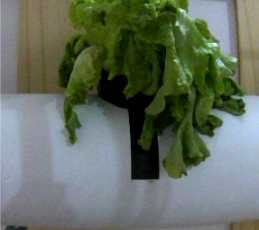
\includegraphics[width=\textwidth]{imagenes/detector_marcadores_1_original.png}
    \caption{Imagen RGB original capturada}
\end{subfigure}
\hfill
\begin{subfigure}[b]{0.48\textwidth}
    \centering
    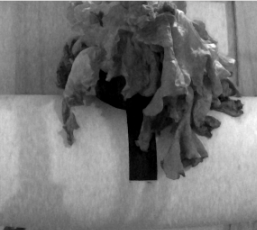
\includegraphics[width=\textwidth]{imagenes/detector_marcadores_2_canal_v.png}
    \caption{Canal V extraído (brillo)}
\end{subfigure}

\vspace{0.3cm}

\begin{subfigure}[b]{0.48\textwidth}
    \centering
    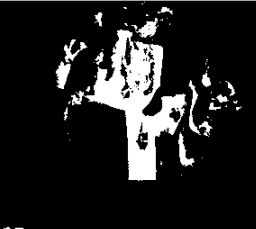
\includegraphics[width=\textwidth]{imagenes/detector_marcadores_3_binario.png}
    \caption{Umbralización binaria inversa (T=50)}
\end{subfigure}
\hfill
\begin{subfigure}[b]{0.48\textwidth}
    \centering
    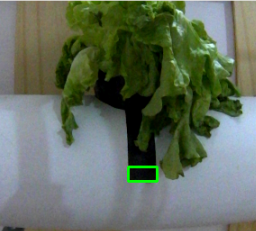
\includegraphics[width=\textwidth]{imagenes/detector_marcadores_4_contornos.png}
    \caption{Contornos detectados con evaluación ponderada}
\end{subfigure}

\caption{\textit{Secuencia de procesamiento del detector de cintas mostrando las transformaciones sucesivas de la imagen}}
\label{fig:proceso_marcadores}
\end{figure}
